\newpage
\subsection{Building of TSEngine}
\label{sec:build}
\hspace{\parindent} The main purpose of creating a sophisticated building system is to assure the project is multiplatform, non-device dependent and is easy to set up.\\ This is necessary for long-living and non-single developer projects.
To fulfill those guidelines, the core of every modern C++ project is CMake, and this is no different in our project.
A comprehensive series of articles about types of libraries in C++ from Medium \textit{"Cpp Libraries"} \cite{cpplibs} can be a great source of knowledge that is useful in this section.
Our building is based on \hyperref[sec:stack_cmake]{\ref*{sec:stack_cmake} CMake} that recently has become the leading tool in building C++ systems.
\subsubsection{Build Structure}
\hspace{\parindent} The following figure shows the build structure of TSEngine:
\label{fig:build_struct}
\begin{figure}[H]
  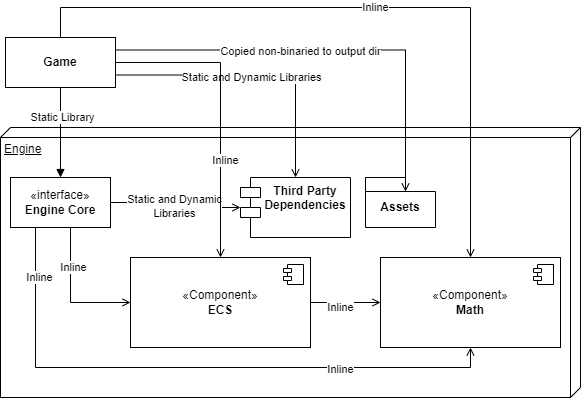
\includegraphics[width=\linewidth]{figures/build.png}
  \caption{Build Structure}
\end{figure}
Currently, TSEngine is delivered to the game part of the project in the form of static library, unfortunately at the moment of writing this thesis we haven't implemented dynamic version of TSEngine yet, but we provided abstraction and architecture to do it.
As the  figure presents, the engine consists of two distinct components: Entity Component System(ECS) and Math libraries which are header only template libraries, both of which can be optionally included to the game.

As it was said in the previous paragraph, for now, the engine can be built only as a static library, and all third party dependencies must be added to the executable.

Assets are copied to the output directory whenever the engine or game is built. This fragment deservers further attention, because it shows a problem while compiling shaders - what mentioned was mentioned in the \hyperref[problem_with_shader_compilation]{\ref*{problem_with_shader_compilation} Shader Compiler} section. However, it would be also advised to store assets in binary packages for the game usage, as it is a common practice nowadays. It, with an addition of serialization of the game structures, would create a pretty functional system.

\begin{verbatim}
├───engine
│   ├───CMakeLists.txt
│   └───tests
│       └───CMakeLists.txt
├───external
│   └───CMakeLists.txt
├───game
│   └───CMakeLists.txt
└───CMakeLists.txt
\end{verbatim}
\begin{table}[h]
\caption{CMake files}
\end{table}
\newpage
\subsubsection{Instruction How To Build the Project}
\hspace{\parindent} Instructions which are needed to build the project:
\label{sec:how_to_run}
\begin{enumerate}
    \item Be sure that you have already installed and updated graphics drivers and your GPU's capabilities are enough - see the section \hyperref[sec:hardware]{\ref*{sec:hardware} Hardware}.
    \item Be sure that you have already installed all the needed VR headset software and set up the environment to play - again, available in the section \hyperref[sec:hardware]{\ref*{sec:hardware} Hardware}.
    \begin{enumerate}
        \item Optional Virtualizer: If you want to use the Virtualizer, be sure to have all needed software installed and set up the treadmill to play.
    \end{enumerate}
    \item Download Git if you don't have yet:
        \href{https://git-scm.com/downloads}{https://git-scm.com/downloads}
    \item Download CMake if you don't have yet:
        \href{https://cmake.org/download/}{https://cmake.org/download/}
    \item Download Visual Studio with C++ workspace if you don't have yet:
        \href{https://visualstudio.microsoft.com/vs/}{https://visualstudio.microsoft.com/vs/}
    \item Open system terminal
    \item Run command (cloning the repository):\\
        \texttt{git clone https://github.com/damian-tomczak/tsengine --recursive \&\& cd tsengine}
    \begin{enumerate}
        \item Optional Virtualizer: If you want to use the Virtualizer, move Cyberith SDK to \texttt{external/CybSDK\_Cpp} or set \texttt{CYBSDK\_DIR} with the path where the SDK is unpacked during TSEngine configuration (\ref{proj_conf})
    \end{enumerate}
    \item Run command (creating working directory):\\
        \texttt{mkdir build \&\& cd build}
    \item Run command (creating project files - on Windows by default Visual Studio project if is installed, othwerwise use \texttt{-G} flag):\\
        \texttt{cmake ..}
    \label{proj_conf}
    \item Build the project with your build system.
    \item Run the project: \texttt{./build/output/tsgame/[BUILD TYPE]/tsgame.[EXECUTABLE FORMAT]}
\end{enumerate}

\newpage
\subsubsection{Third Party Dependencies}
\label{sec:3rdparty}
\hspace{\parindent} We prioritize building from source code over using precompiled binaries.
One of the modern ways of handling compiling from source code is to use git submodules. The core of this method is \texttt{.gitsubmodules} file containing all used external dependencies.
\begin{lstlisting}[caption=.gitsubmodules]
[submodule "external/vulkan"]
	path = external/vulkan
	url = https://github.com/KhronosGroup/Vulkan-Headers.git
[submodule "external/glslang"]
	path = external/glslang
	url = https://github.com/KhronosGroup/glslang
[submodule "external/googletest"]
	path = external/googletest
	url = https://github.com/google/googletest
[submodule "external/openxr"]
	path = external/openxr
	url = https://github.com/KhronosGroup/OpenXR-SDK.git
[submodule "external/tinyobjloader"]
	path = external/tinyobjloader
	url = https://github.com/tinyobjloader/tinyobjloader.git
\end{lstlisting}

The major advantage of source code dependencies over precompiled binaries is having significantly less memory usage to store a project and easy way to make a fork of your dependency. However, the biggest disadvantage of using their source code lies in increased compilation time.

\subsubsection{Cyberith SDK}
\label{sec:build_cybsdk}
\hspace{\parindent} There is one external dependency that git submodules doesn't cover, that dependency is Cybertith SDK, responsible for communication with the Cyberith Virtualizer ELITE 2 treadmill - see the section \hyperref[sec:virtualizer]{\ref*{sec:virtualizer} Virtualizer}. This is the only 3rd party library that is included in the project as a binary and is optional to use.

To use the treadmill, Cyberith SDK must be unpacked to the project, while for its configuration - \hyperref[sec:how_to_run]{\ref*{sec:how_to_run} Instruction How To Buld the Project} section contains elaborated information about it.  

\subsubsection{Precompiled Header}
\hspace{\parindent} To reduce the amount of code which you would have to add in every translation unit, a precompiled header can be used. In our project, we used it to reduce the amount of include directives, so as not to mess up with adding STL for the engine's part.

More systemized and modern substitution of a precompiled header is C++20's Modules. Unfortunately, when we started working on engineering thesis the implementation of it was still in a bad condition, especially when paired with CMake. For the end of 2023 year, it is safe to use Modules with CMake for enthusiast projects, so for an instance in our engine.

\begin{lstlisting}[caption=Adding precompiled header(./engine/CMakeLists.txt)]
target_precompile_headers(${PROJECT_NAME} PUBLIC src/pch.h)
\end{lstlisting}

\subsubsection{Building Operating System Specific}
\label{sec:build_os}
\hspace{\parindent} Multiplatform building is covered by following \texttt{os\_files} function that removes all \texttt{*.cpp} files not designed to be used on platform that is currently used to build the project from the \texttt{SRC\_FILES} variable.
\label{lst:os}
\begin{lstlisting}[caption=\texttt{os\_files} function (./engine/CMakeLists.txt)]
function(os_files files_list_name regex)
    set(files_list ${${files_list_name}})
    list(FILTER files_list EXCLUDE REGEX "src/os/*")

    set(OS_FILES)
    if (WIN32)
        file(GLOB_RECURSE OS_FILES
            src/os/win32/${regex}
        )
    else()
        message(FATAL_ERROR "Not implemented")
    endif()

    list(LENGTH OS_FILES OS_FILES_LENGTH)
    if (OS_FILES_LENGTH EQUAL 0)
        message(FATAL_ERROR "Files specific for your system couldn't be found")
    endif()

    list(APPEND files_list ${OS_FILES})
    set(${files_list_name} ${files_list} PARENT_SCOPE)
endfunction()

file(GLOB_RECURSE SRC_FILES
    src/*.cpp
)

os_files(SRC_FILES *.cpp)
\end{lstlisting}

As we will discuss in the section \hyperref[sec:problems]{\ref{sec:problems} Problems During the Development}, we encountered problems with virtual reality on Linux systems. Therefore to keep the project open for further modifications and good practices, we delivered layers of abstraction, and, where an obvious errors were invoked, with messages pointing out that the following code hadn't yet been implemented for the platform currently being built.

At the level of CMake, this problem is handled by the \texttt{message} function with \texttt{FATAL\_ERROR} argument that stops the configuration of the project.

On the other hand, \texttt{\#error not implemented} preprocessor command secures that code at the level of C++.

\subsubsection{Common ABI}
\label{sec:build_abi}
\hspace{\parindent} When developing any library, it is important to care about application binary interface (ABI), because the user of your product may not be using the same headers used to build your library. It can happen for plenty of reasons, especially when the library is dynamically linked, what is prone to errors.

To avoid it, you must oversee your ABI, we took it into the account but as the project's deadline was coming, exceptions from it had started to appear. One of those exceptions representant is Entity Component System's header file - \texttt{ecs.hpp} where there is not any intermediate interface between ECS's header and the engine prepared.

Therefore to provide at least any kind of protection on top of that we have prepared, \texttt{TS\_VER} preprocessor definition is used as a name of namespace - see the section \hyperref[sec:namespaces]{\ref*{sec:namespaces} Namespaces}. But it is a partial solution, because we must be aware of the fact that a change or addition to the engine breaks the exisiting ABI and we need to update the version of the engine in the main CMake. 

\subsubsection{Preprocess Definitions}
\hspace{\parindent} Publicly exposed engine's preprocessor definitions are: \texttt{ENGINE\_NAME} and \texttt{TS\_VER}.\\ First containing the \texttt{PROJECT\_NAME} variable set as \texttt{tsengine} (so far it is used for creating Khronos's APIs' Instances because they take engine's name). The latter assures \hyperref[sec:build_abi]{\ref{sec:build_abi} Common ABI} works properly.

On the other hand private preprocessor definitions are: \texttt{VK\_USE\_PLATFORM\_\$\{VK\_USE\_PLATFORM\}\_KHR} that is required by Vulkan Headers to choose appropriate declarations based on the system in use, \texttt{VK\_NO\_PROTOTYPES} which is similar to the previous definition as it is related to the Vulkan Headers dependency but this one turns off default Vulkan Loader the dependency comes with - \hyperref[sec:3rdparty]{\ref*{sec:3rdparty} Third Party Dependencies}.\\
\texttt{XR\_USE\_GRAPHICS\_API\_VULKAN} is required for OpenXR to know which graphics API you use, \texttt{CYBSDK\_FOUND} is defined if Cyberith SDK is found - see \hyperref[sec:build_cybsdk]{\ref*{sec:build_cybsdk} Cyberith SDK}, \texttt{TESTER\_ADAPTER} is defined when tests are enabled, which are by default are, and the purpose of \texttt{NOMINMAX} is to disable \texttt{min}, \texttt{max} preprocessor functions defined in Windows API causing problems with STL.
\begin{lstlisting}[caption=Engine's preprocessor definitions (./engine/CMakeLists.txt)]
target_compile_definitions(${PROJECT_NAME} PUBLIC
    ENGINE_NAME="${PROJECT_NAME}"
    TS_VER=v${PROJECT_VERSION_MAJOR}_${PROJECT_VERSION_MINOR}_${PROJECT_VERSION_PATCH}
)

...

target_compile_definitions(${PROJECT_NAME} PRIVATE
    VK_USE_PLATFORM_${VK_USE_PLATFORM}_KHR
    VK_NO_PROTOTYPES
    XR_USE_GRAPHICS_API_VULKAN
    $<$<BOOL:${CYBSDK_LIB}>:CYBSDK_FOUND>
    $<$<BOOL:${ENABLE_TESTS}>:TESTER_ADAPTER>
    $<$<PLATFORM_ID:Windows>:NOMINMAX>
)
\end{lstlisting}

If we are talking about the game's preprocessor definitions, we are not dealing with a list but a single definition - \texttt{GAME\_NAME} storing the name of the game created with the help of the engine. It is also used for setting Khronos's APIs and among others, window's name.
\begin{lstlisting}[caption=Game's preprocessor definitions (./game/CMakeLists.txt)]
target_compile_definitions(${PROJECT_NAME} PUBLIC
    GAME_NAME="${GAME_NAME}"
)
\end{lstlisting}

\label{game_name}
The name setup of the game happens during the project configuration, so the change of the default name "Awesome Game" must be done by providing the \texttt{-DGAME\_NAME="Non-default game name"} flag to the project configuration.
\begin{lstlisting}[caption=Game's preprocessor definitions (./CMakeLists.txt)]
set(GAME_NAME "Awesome Game" CACHE STRING "Game name")
message(STATUS "Game name: ${GAME_NAME}")
\end{lstlisting}

\subsubsection{Included Directories}
\hspace{\parindent} Decision about which directories are included to the project at the first glance may seem to be childish topic to discuss, but in practice, not thoughtfully made decision in this aspect can be very dangerous for the development and from the long-term perspective destroy the project. It is important only add to the project paths which clearly represent which modules they open access to.

Taking into the account those reasons, relative included directories should be avoided.
Following code snippet shows which paths are explicitly added to the project:
\label{lst:exp_incl}
\begin{lstlisting}[caption=Explicitly included directories (./engine/CMakeLists.txt)]
target_include_directories(${PROJECT_NAME} PUBLIC
    include
)

...

target_include_directories(${PROJECT_NAME} PRIVATE
    src
    ${OS_DIR}
    ${EXTERNAL_DIR}/glslang
    ${CYBSDK_INCLUDE_DIR}
    ${ASSETS_DIR}
)
\end{lstlisting}

It should be remembered that plenty of included directories are added by modern CMake's approach where operation of adding the headers happens while linking libraries: 
\begin{lstlisting}[caption=Implicitly added directories (./engine/CMakeLists.txt)]
target_link_libraries(${PROJECT_NAME} PUBLIC
    Vulkan-Headers
    glslang
    SPIRV
    openxr_loader
    headers
    tinyobjloader
    ${CYBSDK_LIB}
)
\end{lstlisting}
The only corner case here is glslang dependency that requires to be added manually because it doesn't support modern approach.

\subsubsection{Unit Tests}
\label{sec:build_unit_tests}
\hspace{\parindent} One of the methods of testing the software are unit tests - elaborated further in the \hyperref[sec:testing]{\ref*{sec:testing} Software Testing} section. This is the method we have chosen for testing our project.
Deeper deliberation about unit tests in TSEngine consisting of, among other things, a list of those and the purpose of each one of them, can be found in the section dedicated to it, namely \hyperref[sec:tests]{\ref*{sec:tests} Tests}.

Following code listing presents adding groups of tests for the testing, however, tests from \texttt{GameTests} group are added in a different way, because it happens only when the  \texttt{CI\_RUNNING} variable is set to \texttt{false}.
Further discussion about this variable can be found in \texttt{./.github/workflows/.cmake.yml} code listing from the next subsubsection - \hyperref[sec:scv]{\ref*{sec:scv} Source Control Version}.
\begin{lstlisting}[caption=Adding tests to CTest (./engine/CMakeLists.txt)]
add_test(DummyTests ${PROJECT_NAME} --gtest_filter=DummyTests.*)
add_test(MathTests ${PROJECT_NAME} --gtest_filter=MathTests.*)

option(CI_RUNNING "" OFF)

if(NOT CI_RUNNING)
    add_test(GameTests ${PROJECT_NAME} --gtest_filter=GameTests.*)
endif()
\end{lstlisting}

\begin{lstlisting}[caption=Enabling Tests(./CMakeLists.txt)]
option(ENABLE_TESTS "Test the engine basic operations" ON)
\end{lstlisting}

\begin{lstlisting}[caption=\texttt{TESTER\_ADAPTER} preprocessor declaration(./engine/CMakeLists.txt and ./engine/tests/CMakeLists.txt)]
target_compile_definitions(${PROJECT_NAME} PRIVATE
    ...
    $<$<BOOL:${ENABLE_TESTS}>:TESTER_ADAPTER>
)
\end{lstlisting}

We are not satisfied with our implementation of \texttt{TesterEngine} header, that gives utils needed while testing the engine. It's extremely dangerous to expose all the engine for tests, they should have access only to functionalities available for the games. It will be fixed soon. 
\begin{lstlisting}[caption=Including common internal utils (./engine/tests/CMakeLists.txt)]
target_include_directories(${PROJECT_NAME} PRIVATE
    ../src
)
\end{lstlisting}

\subsubsection{Source Control Version}
\label{sec:scv}
\hspace{\parindent}
Even if a project is not done as a team, or there are no plans for long-term development it is worth to use source control version system, because it may turn out that the assumptions about the project may change, or you can encounter a regression that can be easily fixed with SCV system.  Nowadays, it is not possible for the project not to have source control version system. It is further explained in section \hyperref[sec:teamwork]{\ref*{sec:teamwork} Teamwork}.
We decided to use GIT as our SVC, with GitHub as remote server:

\label{lst:cicmake}
Continuous integration is extremely useful for avoiding regression in a product. In our case, we used CI to test only if the project builds and passes unit tests:
\begin{lstlisting}[caption=Continuous intergration build test (./.github/workflows/.cmake.yml)]
name: CMake

on:
  push:
    branches: [ "master" ]
  pull_request:
    branches: [ "master" ]

env:
  BUILD_TYPE: Release

jobs:
  build:
    runs-on: windows-latest

    steps:
    - uses: actions/checkout@v3

    - name: Update submodules
      run: git submodule update --init --recursive

    - name: Configure CMake
      run: cmake -B ${{github.workspace}}/build -DCMAKE_BUILD_TYPE=${{env.BUILD_TYPE}} -DCI_RUNNING=ON

    - name: Build
      run: cmake --build ${{github.workspace}}/build --config ${{env.BUILD_TYPE}}

    - name: Test
      working-directory: ${{github.workspace}}/build/engine
      run: ctest -C ${{env.BUILD_TYPE}}
\end{lstlisting}
Every push and pull request to the \texttt{master} branch invokes a job in which a remote machine tests if configuration of CMake and building the project in \texttt{RELEASE} build type is successful, otherwise an action requested is declined.

As we're describing SCV, it's worth to mention our \texttt{.gitignore} file that assumes \texttt{build} directory will be the working directory, VS Code will be our helper code editor (it's worth to ignore \texttt{.vscode} dir as it is often unwantedly created by this code editor), subdirectories of \texttt{external}, as so far we didn't want to make any changes to our external dependencies.
\label{lst:gitignore}
\begin{lstlisting}[caption=\texttt{.gitignore} (./.gitignore)]
build
.vscode
external/*/
\end{lstlisting}